\documentclass[xcolor=x11names,compress]{beamer}

%% General document %%%%%%%%%%%%%%%%%%%%%%%%%%%%%%%%%%
\usepackage{graphicx}
\usepackage{tikz}
\usepackage{Tabbing}
\usetikzlibrary{decorations.fractals}
\usepackage{fancyvrb}
%%%%%%%%%%%%%%%%%%%%%%%%%%%%%%%%%%%%%%%%%%%%%%%%%%%%%%

%% Beamer Layout %%%%%%%%%%%%%%%%%%%%%%%%%%%%%%%%%%
\useoutertheme[subsection=false,shadow]{miniframes}
\useinnertheme{default}
\usefonttheme{serif}
\usepackage{palatino}
\usepackage{tabu}
% Links
\usepackage{hyperref}
\definecolor{links}{HTML}{003262}
\hypersetup{colorlinks,linkcolor=,urlcolor=links}

% addition of color
\usepackage{xcolor}
\definecolor{CoolBlack}{rgb}{0.0, 0.18, 0.39}
\definecolor{byellow}{rgb}{0.55037, 0.38821, 0.06142}
\definecolor{dgreen}{rgb}{0.,0.6,0.}
\definecolor{RawSienna}{cmyk}{0,0.72,1,0.45}
\definecolor{forestgreen(web)}{rgb}{0.13, 0.55, 0.13}
\definecolor{cardinal}{rgb}{0.77, 0.12, 0.23}

\setbeamerfont{title like}{shape=\scshape}
\setbeamerfont{frametitle}{shape=\scshape}

\setbeamercolor*{lower separation line head}{bg=CoolBlack} 
\setbeamercolor*{normal text}{fg=black,bg=white} 
\setbeamercolor*{alerted text}{fg=dgreen} % just testing; I think this looks better
\setbeamercolor*{example text}{fg=black} 
\setbeamercolor*{structure}{fg=black} 
 
\setbeamercolor*{palette tertiary}{fg=black,bg=black!10} 
\setbeamercolor*{palette quaternary}{fg=black,bg=black!10} 

% Margins
\usepackage{changepage}

\mode<presentation>
{
  \definecolor{berkeleyblue}{HTML}{003262}
  \definecolor{berkeleygold}{HTML}{FDB515}
  \usetheme{Boadilla}      % or try Darmstadt, Madrid, Warsaw, Boadilla...
  %\usecolortheme{dove} % or try albatross, beaver, crane, ...
  \setbeamercolor{structure}{fg=berkeleyblue,bg=berkeleygold}
  \setbeamercolor{palette primary}{bg=berkeleyblue,fg=white} % changed this
  \setbeamercolor{palette secondary}{fg=berkeleyblue,bg=berkeleygold} % changed this
  \setbeamercolor{palette tertiary}{bg=berkeleyblue,fg=white} % changed this
  \usefonttheme{structurebold}  % or try serif, structurebold, ...
  \useinnertheme{circles}
  \setbeamertemplate{navigation symbols}{}
  \setbeamertemplate{caption}[numbered]
  \usebackgroundtemplate{}
}

% Columns
\renewcommand{\(}{\begin{columns}}
\renewcommand{\)}{\end{columns}}
\newcommand{\<}[1]{\begin{column}{#1}}
\renewcommand{\>}{\end{column}}

\usepackage{cutwin}

% adding slide numbers
\addtobeamertemplate{navigation symbols}{}{%
    \usebeamerfont{footline}%
    \usebeamercolor[fg]{footline}%
    \hspace{1em}%
    \insertframenumber/\inserttotalframenumber
}

% equation stuff
\newcommand{\Macro}{\ensuremath{\Sigma}}
\newcommand{\Sn}{\ensuremath{S_N} }
\newcommand{\vOmega}{\ensuremath{\hat{\Omega}}}
\usepackage{mathrsfs}
\usepackage[mathcal]{euscript}
\usepackage{amssymb}
\usepackage{amsthm}
\usepackage{epsfig}
\usepackage{amsmath}
\newcommand{\ve}[1]{\ensuremath{\mathbf{#1}}}
\newcommand{\micro}{\ensuremath{\sigma}}
\newcommand{\detR}{\ensuremath{\Sigma}}

% title stuff for footer
\title{Methods and Software in NE}
\author{R.\ N.\ Slaybaugh}
\date{4 December 2014}

%%%%%%%%%%%%%%%%%%%%%%%%%%%%%%%%%%%%%%%%%%%%%%%%%%%%%%
\begin{document}



%%%%%%%%%%%%%%%%%%%%%%%%%%%%%%%%%%%%%%%%%%%%%%%%%%%%%%
%%%%%%%%%%%%%%%%%%%%%%%%%%%%%%%%%%%%%%%%%%%%%%%%%%%%%%
\begin{frame}
\title{Computational methods and software development }
\subtitle{in nuclear engineering research}
\author{
        \includegraphics[height=2cm]{../bk-eps-converted-to}\\R.\ N.\ Slaybaugh \\ Univ.\ of Cal.\ Berkeley}

\date{BIDS Tea \\ 3 December 2014}
\titlepage
\end{frame}

%------------------------------------------------------
\begin{frame}{What Are We Sovling?}

    I study how to solve the steady state, neutral particle Boltzmann transport equation
    more efficiently:
    %   
    \begin{align}
    [\vOmega \cdot \nabla + \Macro(\vec{r}, E)] &\psi(\vec{r}, \vOmega, E)  =  + q(\vec{r}, \vOmega, E) \nonumber\\
     &\int_0^{\infty} dE' \int_{4\pi} d\vOmega' \:\Macro_{s}(\vec{r}, E' \to E,
     \vOmega' \cdot \vOmega) \psi(\vec{r}, \vOmega', E') \nonumber
    \end{align}

    Discretize, then convert to operator form:
    \begin{align}
    \mathbf{L} \psi &= \mathbf{MS}\phi + \mathbf{Q} \nonumber\\
    \phi &= \mathbf{D}\psi \nonumber \\
    \underbrace{(\ve{I} - \ve{DL}^{-1}\ve{MS})}_{\mathbf{A}}\phi &= \mathbf{Q}\nonumber
    \end{align}
    
    \textcolor{dgreen}{Properties of the matrix} govern solution behavior
    
\end{frame}


%------------------------------------------------------
\begin{frame}{Properties Affect Solver Choice}

    \begin{columns}
    \begin{column}{0.45\textwidth}
     
        \textcolor{dgreen}{Properties of the matrix} influence solver choices
        \begin{itemize}
        \item Inner iteration methods
        \item Outer iteration methods
        \item Eigenvalue iteration methods
        \item Preconditioners
        \end{itemize}
    
        Method choices are also driven by \textcolor{dgreen}{hardware} considerations
  	\end{column}
   	%
 	\begin{column}{0.45\textwidth}
 	   \begin{center}
 	   \begin{figure}
 	   \includegraphics[height=2.75in,clip]{../2014-10-norcalANS/solverLayers}
       \end{figure}
 	   \end{center}
  	\end{column}
	\end{columns}
	
\end{frame}
% All of the discretization choices and all of the solution stratgies create a complex set of choices

%------------------------------------------------------
\begin{frame}{Algorithms + Architecture + Application}

    \begin{columns}
    \begin{column}{0.5\textwidth}
    
 	   \begin{center}
 	   \begin{figure}     
 	   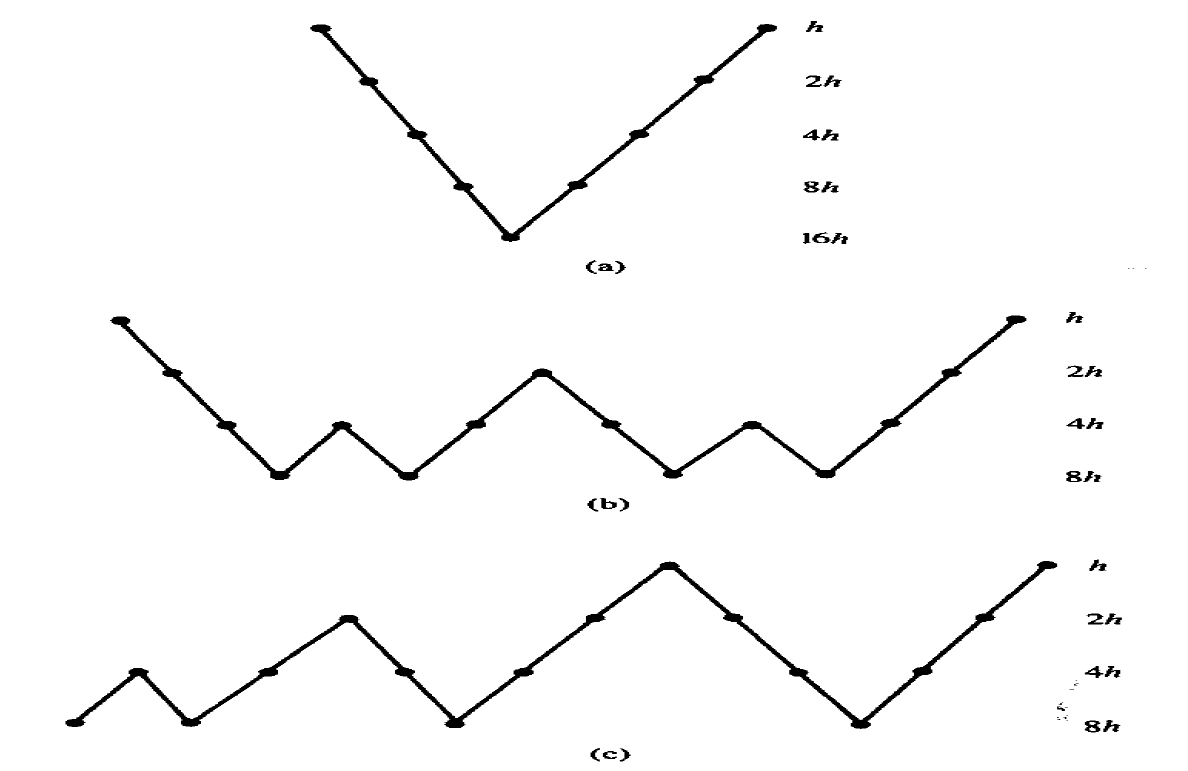
\includegraphics[height=1.25in, width=1.25in, clip]{../figs/multigridFig}
 	   \end{figure}
 	   \begin{figure} 
 	   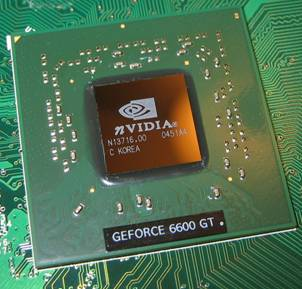
\includegraphics[height=1in,clip]{../figs/GPU}
       \end{figure}
 	   \end{center}

  	\end{column}
   	%
 	\begin{column}{0.5\textwidth}
 	   \begin{center}
 	   \begin{figure}
 	   \includegraphics[height=2.75in,clip]{../figs/PWR-maps}
       \end{figure}
 	   \end{center}
  	\end{column}
	\end{columns}
	
\end{frame}

%%%%%%%%%%%%%%%%%%%%%%%%%%%%%%%%%%%%%%%%%%%%%%%%%%%%%%
%%%%%%%%%%%%%%%%%%%%%%%%%%%%%%%%%%%%%%%%%%%%%%%%%%%%%%
\begin{frame}{What is PyNE?}

    PyNE is an open source \alert{library of composable tools} used to build 
    nuclear science and engineering applications. \\
    \textbf{Goals:}
    
    \begin{columns}
    \begin{column}{0.45\textwidth}
        \begin{itemize}
        \item be more \alert{productive} (don't reinvent the wheel!)
        \item have the \alert{best solvers}
        \item have a clear and useful API
        \item write really \alert{great code}
        \item \alert{teach} the next generation
        \end{itemize}
    It is permissively licensed (2-clause BSD)\\
    \vspace{0.5 em}
    It supports both a \alert{C++} and a \textcolor{dgreen}{Python} API
  	\end{column}
   	%
 	\begin{column}{0.45\textwidth}
 	   \begin{center}
 	   \begin{figure}
       \includegraphics[height=4cm]{../figs/pyne-icon-big}
	   \end{figure}
 	   \end{center}
  	\end{column}
	\end{columns}

\end{frame}

%%%%%%%%%%%%%%%%%%%%%%%%%%%%%%%%%%%%%%%%%%%%%%%%%%%%%%
%%%%%%%%%%%%%%%%%%%%%%%%%%%%%%%%%%%%%%%%%%%%%%%%%%%%%%
\section{PyNE as a research tool}  
\begin{frame}{PyNE as a research tool}

    \textbf{Insight}: PyNE lets us access the physics, have real materials, 
    add mesh, and handle many details easily...

    \vspace{2 em}
    \textbf{Idea}: perfect environment for investigating numerical methods that 
    are impacted by materials, mesh, etc. 

    \vspace{2 em}
    \textbf{My Plan:} Plug-And-Play Solver Research Environment
    
\end{frame}



%------------------------------------------------------
\begin{frame}{Plug-And-Play Research Environment}

    Make collections of \textcolor{dgreen}{interchangeable pieces} for each component
    needed to construct a transport solver
    
    \vspace*{1em}
    Researchers can then 
    \begin{itemize}
    \item \textcolor{dgreen}{Assemble} a transport solver to fit their needs
    \item \textcolor{dgreen}{Add} their own new methods and investigate how 
    they interact with different solver combinations
    \end{itemize}

    \vspace*{1em}
    Implementing this in PyNE provides access to 
    \begin{itemize}
    \item PyNE's \textcolor{dgreen}{resources} such as nuclear data, materials, 
    and mesh tools  
    \item A flexible and robust \textcolor{dgreen}{development environment} 
    \item A well-managed \textcolor{dgreen}{API}
    \end{itemize}

\end{frame}

% --------------------------------------------------------------
%\begin{frame}[allowframebreaks]{References}
%	\bibliographystyle{unsrt}
%	\bibliography{pynepubs.bib}
%\end{frame}

\end{document}
